\documentclass[../../main]{subfiles}

\renewcommand\thesection{\arabic{section}}


\begin{document}

\section{Micro Climate Management} \label{sec:}

\begin{minipage} {0.62\textwidth}
    \vspace{-0.8cm}

    Developed a TinyML-based greenhouse monitoring system that is deployable on
    most modern microcontrollers. Uing sensor data from a custom strawberry greenhouse
    and a five-action multi-label control strategy, trained and cross-validated 90
    MLPs to identify the most efficient model. And resulted with a performant
    TinyML model.

\end{minipage}
\hfill
\begin{minipage} {0.35\textwidth}
    \begin{center}
        \vspace{-1.2cm}
        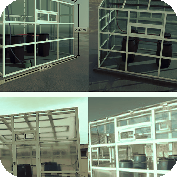
\includegraphics[width = 0.89\textwidth] {pics/microclimate.pdf}
        \captionof{figure}[The experimental greenhouse.]{}
        \label{fig:case2Pic}
    \end{center}
\end{minipage}

\subsection{What They Did}

In this study\cite{microclimate}, researchers developed an optimized tinyML-oriented
model for an active machine learning based greenhouse microclimate management system
to be integrated in an on-field microcontroller. Inorder to collect multivariate climate data,
they designed and deployed an experimental strawberry greenhouse.
Then the dataset is used to train and five-fold cross-validate 90 Multi Layer Perceptrons (MLPs)
with varied hyperparameters and selected the most performant yet optimized model instance for the addressed task.
Figure \ref{fig:case2Pic} shows the experimental greenhouse.

\subsection{Results They Got}

From their 90 model instances, they selected a model incorporated 2 hidden
layers with 7 and 8 neurons respectively and 151 parameters, and it scored a
mean accuracy of 97\% during the cross-validation phase, then 96\% on the
supplementary test set. Thanks to the TinyML approach the developed model
was a light weight one. So it can be effectively deployed on microcontrollers
within real world operating conditions.

\end{document}
